\newpage
\section{Programmation noyau : Module noyau}
\subsection{Module noyau}
\subsubsection{Exercice 1}
\textbf{Donnée : } Générer un module noyau "out of tree" pour la cible ODROID-XU3\\
\textbf{Point a :} Créer	le	squelette	d’un	module	noyau	et	générer	le	en	dehors	des	sources	du	noyau	à	l’aide	d’un	Makefile.	Le	module	devra	afficher	un	message	lors	de	son	enregistrement	et	lors	de	sa	désinstallation.\\\\
\textbf{Emplacement du code : } \textit{/ModulesNoyau/exercice1-Module/pointA}\\
Le code a été écrit conformément aux exemples présentés dans le support de cours.\\

\textbf{Exécution du code : } \\
Le code doit être compilé sur la machine hôte à l'aide de la commande suivante:
\begin{lstlisting}
$ make clean all
\end{lstlisting}

\textbf{Point b :} Tester sur la machine hôte la commande "modinfo" sur	votre	skelette de	module et comparer les	informations retournées	avec celles	du	code source.
\begin{lstlisting}
$ modinfo mymodule.ko
filename:       /home/lmi/workspace/csel1/environment/module_noyau/exercice1/pointa/mymodule.ko
license:        GPL
description:    Module Skeleton
author:         Emilie Gsponer
depends:        
vermagic:       3.10.63 SMP preempt mod_unload ARMv7 p2v8 
\end{lstlisting}
Ces informations correspondent à celles entrée dans le skeleton du module:
\begin{lstlisting}
MODULE_AUTHOR("Emilie Gsponer");
MODULE_DESCRIPTION("Module Skeleton");
MODULE_LICENSE("GPL");
\end{lstlisting}
\textbf{Point c :} Installer	le	module (insmod),	contrôler	le	log	du	noyau	(dmesg).\\\\
\textbf{Exécution du code : }Le module doit être installé sur la cible à l'aide la commande \textit{insmod}. On peut observer que le module a bien été installé à l'aide de la commande \textit{dmesg}.
\begin{lstlisting}
# insmod mymodule.ko
# dmesg | tail -n 4
[    7.704536] [c5] Freeing unused kernel memory: 436K (c089c000 - c0909000)
[    7.877462] [c4] EXT4-fs (mmcblk0p1): re-mounted. Opts: errors=remount-ro,data=ordered
[    8.967876] [c7] pwm-samsung: tin parent at 66600000
[   53.629226] [c4] Linux module skeleton loaded

\end{lstlisting}
\textbf{Point d :} Comparer	les	résultats	obtenus	par	la	commande	"lsmod"	avec	ceux	obtenus	avec	la	commande	"cat /proc/modules".\\\\
\textbf{Exécution des commandes : } Les deux commandes présentent le même résultat, seule la mise en forme est différente.
\begin{lstlisting}
# cat /proc/modules
mymodule 687 0 - Live 0xbf004000 (O)

# lsmod mymodule.ko
Module                  Size  Used by    Tainted: G  
mymodule                 687  0 
\end{lstlisting}
\textbf{Point e :} Désinstaller	le	module	(rmmod).\\\\
\textbf{Exécution de la commande : } On peut voir à l'aide des commandes \textit{cat /proc/modules}, \textit{lsmod} et \textit{dmesg} que le module a bien été désinstallé.
\begin{lstlisting}
# rmmod mymodule
# cat /proc/modules
# lsmod mymodule.ko
Module                  Size  Used by    Tainted: G  
# dmesg | tail -n 4
[    7.877462] [c4] EXT4-fs (mmcblk0p1): re-mounted. Opts: errors=remount-ro,data=ordered
[    8.967876] [c7] pwm-samsung: tin parent at 66600000
[   53.629226] [c4] Linux module skeleton loaded
[   73.538490] [c5] Linux module skeleton unloaded
\end{lstlisting}

\textbf{Point f :} Adapter	le	Makefile	du	module	pour	autoriser	l’installation	du	module	avec	les	autres	modules	du	noyau	permettant	l’utilisation	de	la	commande	"modprobe".	Le	module	devra	être	installé	dans	le	root	filesystem	utilisé	en	nfs	par	la	cible.\\\\
\textbf{Emplacement du code : } \textit{/ModulesNoyau/exercice1-Module/pointF}\\\\
Pour que le module puisse être ajouté dans le noyau, il suffit d'ajouter les lignes suivantes au Makefile:
\begin{lstlisting}
MODPATH := /tftpboot/odroidxu3

install:
$(MAKE) -C $(KDIR) M=$(PWD) INSTALL_MOD_PATH=$(MODPATH) modules_install
\end{lstlisting}
\textbf{Exécution du code : }Le code doit être compilé et installé depuis la machine hôte à l'aide des commandes suivantes:
\begin{lstlisting}
$ make clean all
$ sudo make install
\end{lstlisting}
Il faut ensuite démarrer la cible en mode nfs pour y installer le module à l'aide de la commande \textit{modprobe}
\begin{lstlisting}
lmi@csel1:~/.ssh$ sudo minicom
...
ODROIDXU3> run nfsboot
(Re)start USB...
...
Welcome to Hardkernel ODROID_XU3 board                                          
odroidxu3 login: root  
# modprobe mymodule                                                             
[   98.024580] [c2] Linux module skeleton loaded                                
# modprobe -r mymodule                                                          
[   99.673514] [c0] Linux module skeleton unloaded   
\end{lstlisting}
\subsubsection{Exercice 2}
\textbf{Donnée : } Adapter	le	module	de	l’exercice	précédent	afin	qu’il	puisse	recevoir	deux	ou	trois paramètres de	votre	choix.	Ces	paramètres	seront	affichés dans	la	console.	Adapter	également	le rootfs	afin	de	pouvoir	utiliser	la	commande	"modprobe".\\\\
\textbf{Emplacement du code : } \textit{/ModulesNoyau/exercice2-Parameter}\\\\
\textbf{Exécution du code : }Ce module prend deux paramètres d'entrée par défaut, text = "hello" et elements = 2. La valeur de ces éléments peut être modifiée lors de l'installation du module dans le noyau, comme le montre la démonstration suivante.
\begin{lstlisting}
# modprobe mymodule                                                             
[  922.323941] [c1] Linux module skeleton loaded                                
[  922.326835] [c1] text:hello                                                  
[  922.326835] elements:2                                                       
# modprobe -r mymodule                                                          
[  925.223513] [c0] Linux module skeleton unloaded                         
# modprobe mymodule text="hello world" elements=10                              
[ 1196.597223] [c2] Linux module skeleton loaded                                
[ 1196.600182] [c2] text:hello world                                            
[ 1196.600182] elements:10                                                      
# modprobe -r mymodule                                                          
[ 1199.518513] [c0] Linux module skeleton unloaded  
\end{lstlisting}
\textbf{Remarque : } Pour tous les exercices suivants, on reprendra le même Makefile permettant d'installer le module directement dans le noyau à l'aide de la commande \textit{modprobe}. Il faudra pour cela que la cible soit démarrée en mode nfs. Le module de chaque exercice devra être compilé et installé à l'aide des commandes suivantes:
\begin{lstlisting}
$ make clean all
$ sudo make install
\end{lstlisting}
\subsubsection{Exercice 3}
\textbf{Donnée : } Trouver	la	signification	des	4	valeurs	affichées	lorsque	l’on	tape	la	commande "cat /proc/sys/kernel/printk".\\\\
\textbf{Exécution de la commande : }
\begin{lstlisting}
# cat /proc/sys/kernel/printk                                                   
10      4       1       7 
\end{lstlisting}
Ces chiffres représentent le log level du kernel utilisé pour déterminer l'importance d'un message.
\begin{enumerate}
	\item 10 : current loglevel
	\item 4 : default loglevel
	\item 1 : minimum loglevel
	\item 7 : boot-time-default loglevel
\end{enumerate}
Cela permet de définir la priorité des messages. Si un message a une priorité plus grande (chiffre plus petit) que le loglevel courant du kernel, il sera affiché dans la console. Dans le cas contraire, le message n'est pas affiché.L'exemple suivant le démontre en passant le loglevel à 1, le module n'affiche plus de message dans la console.
\begin{lstlisting}
# echo 10 > /proc/sys/kernel/printk                                             
# cat /proc/sys/kernel/printk                                                   
10      4       1       7                                                       
# modprobe mymodule                                                             
[ 2139.129459] [c2] Linux module skeleton loaded                                
[ 2139.132348] [c2] text:hello                                                  
[ 2139.132348] elements:2                                                       
# modprobe -r mymodule                                                          
[ 2143.683511] [c0] Linux module skeleton unloaded        
                      
# echo 1 > /proc/sys/kernel/printk                                              
# cat /proc/sys/kernel/printk                                                   
1       4       1       7                                                       
# modprobe mymodule                                                             
# modprobe -r mymodule     
                                                     
# echo 10 > /proc/sys/kernel/printk                                             
# modprobe mymodule                                                             
[ 2173.021095] [c2] Linux module skeleton loaded                                
[ 2173.024050] [c2] text:hello                                                  
[ 2173.024050] elements:2    
\end{lstlisting}  
Source : \url{http://elinux.org/Debugging_by_printing}

\subsection{Gestion de la mémoire, bibliothèques et fonctions utiles}
\subsubsection{Exercice 4}
\noindent
\textbf{Donnée : }Créer dynamiquement des éléments dans le noyau. Adapter un module noyau afin que l'on puisse lors de son installation spécifier un nombre d'éléments à créer ainsi qu'un texte initial à stocker dans les éléments précédemment alloués. Chaque élément contiendra également un numéro unique, Les éléments seront créés lors de l'installation du module et chainés dans une liste. Ces éléments seront détruits lors de la désinstallation du module. Des messages d'information seront émis afin de permettre le debugging du module.\\\\
\textbf{Emplacement du code : } \textit{/ModulesNoyau/exercice4-List}\\\\
\textbf{Exécution du code : }
\begin{lstlisting}
# modprobe mymodule element_num=5 text="Hello world"                            
[ 2250.418060] [c2] New element added to the list                               
[ 2250.421107] [c2] New element added to the list                               
[ 2250.425536] [c2] New element added to the list                               
[ 2250.429937] [c2] New element added to the list                               
[ 2250.434368] [c2] New element added to the list                               
[ 2250.438773] [c2] ID of element : 0                                           
[ 2250.438773] String is : Hello world                                          
[ 2250.445642] [c2] ID of element : 1                                           
[ 2250.445642] String is : Hello world                                          
[ 2250.452489] [c2] ID of element : 2                                           
[ 2250.452489] String is : Hello world                                          
[ 2250.459415] [c7] ID of element : 3                                           
[ 2250.459415] String is : Hello world                                          
[ 2250.466444] [c7] ID of element : 4                                           
[ 2250.466444] String is : Hello world                                          
# modprobe -r  mymodule                                                         
[ 2267.933575] [c1] Element poped                                               
[ 2267.935161] [c1] Element poped                                               
[ 2267.938196] [c1] Element poped                                               
[ 2267.941283] [c1] Element poped                                               
[ 2267.944313] [c1] Element poped                                               
[ 2267.947308] [c1] Module removed
\end{lstlisting}
\subsubsection{Exercice 5}
\noindent
\textbf{Donnée : }Indiquer les différents alocateurs SLAB disponibles dans le noyau Linux pour la cible ORDOID-XU3.\\\\
\textbf{Réponse:}
\begin{enumerate}
	\item SLAB : "as cache frendly as possible, benchmark frendly"
	\item SLOB : "as compact as possible"
	\item SLUB : "Simple and instruction cost counts. Superior Debugging. Defragmentation. Execution time friendly"
\end{enumerate}
Source : \url{https://www.google.ch/url?sa=t&rct=j&q=&esrc=s&source=web&cd=3&cad=rja&uact=8&ved=0CDEQFjACahUKEwiqj6GfhKbIAhWLXBoKHXDUAow&url=http%3A%2F%2Fwww.cs.berkeley.edu%2F~kubitron%2Fcourses%2Fcs194-24-S14%2Fhand-outs%2Fbonwick_slab.pdf&usg=AFQjCNENx6yGi8dVRbdR2Si1OpXE_NuNkg&sig2=ZdJ_jUWHIfO1qFIIikEyHA}
	
\subsection{Accès aux entrées/sorties}
\subsubsection{Exercice 6}
\textbf{Donnée : }À l'aide d'un module noyau, réserver la zone mémoire correspondante au registre du uP décrivant son identification. Adress de départ 0x1000'0000, taille de la zone 0x100. Valider cette réservation à l'aide de la commande "cat /proc/iomem".\\
\\
Adapter ce module afin d'afficher cet identifiant dans la console de déboggage "dmesg". Ce dernier est composé des champs suivants:
\begin{enumerate}
	\item Bit 31..12: product id
	\item Bit 11..8: package id
	\item Bit 7..4: major revision
	\item Bit 3..0: minor revision\\
\end{enumerate}
\textbf{Emplacement du code : } \textit{/ModulesNoyau/exercice6-IO}\\\\
\textbf{Complément : }L'identifiant demandé par la donnée est en fait l'identifiant de la zone mémoire réservée. Il peut être obtenu grâce à la méthode \textit{ioread}. Mais pour pouvoir lire cette zone, il faut la mapper dans la mémoire virtuelle du noyau avec la méthode \textit{ioremap}, car le noyau n'a pas directement accès aux entrées/sorties.\\
La zone mémoire réservée par le code a été nommée "uP register".\\\\
\textbf{Exécution du code : }
\begin{lstlisting}
# modprobe mymodule                                                             
[   30.336553] [c5] Linux module skeleton loaded                                
[   30.339495] [c5] Memory allocated                                            
[   30.342733] [c5] uP register: Bit 31..12 : product id=0x65422                
[   30.348494] [c5] uP register: Bit 11..8  : package id=0x0                    
[   30.353877] [c5] uP register: Bit 7..4   : major revision=0x0                
[   30.359597] [c5] uP register: Bit 3..0   : minor revision=0x1                
# cat /proc/iomem                                                               
03000000-03048fff : /lpass@03810000                                             
03810000-038100ff : /lpass@03810000                                             
03830000-038300ff : samsung-i2s                                                 
03860000-03860fff : /pinctrl@03860000                                           
03880000-03880fff : /amba/adma@03880000                                         
03880000-03880fff : /amba/adma@03880000                                      
10000000-100000ff : uP register                                                 
...                                             
# dmesg |tail -n 10                                                             
[    9.041140] [c4] VFS: Mounted root (nfs filesystem) on device 0:13.          
[    9.048765] [c4] devtmpfs: mounted                                           
[    9.050869] [c4] Freeing unused kernel memory: 436K (c089c000 - c0909000)    
[   12.571761] [c4] pwm-samsung: tin parent at 66600000                         
[   30.336553] [c5] Linux module skeleton loaded                                
[   30.339495] [c5] Memory allocated                                            
[   30.342733] [c5] uP register: Bit 31..12 : product id=0x65422                
[   30.348494] [c5] uP register: Bit 11..8  : package id=0x0                    
[   30.353877] [c5] uP register: Bit 7..4   : major revision=0x0                
[   30.359597] [c5] uP register: Bit 3..0   : minor revision=0x1                
# modprobe -r  mymodule                                                         
[   88.338556] [c0] Linux module skeleton unloaded                              
[   88.341621] [c0] Memory released    
\end{lstlisting}

\subsection{Threads du noyau}
\subsubsection{Exercice 7}
\textbf{Donnée : }Développer	un	petit	module	permettant	d’instancier	un	thread	dans	le	noyau.	Ce	thread	affichera	un	message	toutes	les	5	secondes.	Il	pourra	être	mis	en	sommeil	durant	ces	5	secondes à	l’aide	de	la	fonction	« ssleep(5) »	provenant	de	l’interface	<linux/delay.h>.\\\\
\textbf{Emplacement du code : } \textit{/ModulesNoyau/exercice7-Thread}\\\\
\textbf{Exécution du code : }
\begin{lstlisting}
# modprobe mymodule                                                             
[ 1434.469821] [c2] Thread created                                              
# [ 1439.473573] [c1] Thread awake                                              
[ 1444.478588] [c2] Thread awake                                                
[ 1449.483589] [c3] Thread awake                                                
# modprobe -r  mymodule                                                         
[ 1454.488597] [c0] Thread awake                                                
[ 1454.490139] [c1] Thread stopped   
\end{lstlisting}
\subsection{Mise en sommeil}
\subsubsection{Exercice 8}
\textbf{Donnée : }Développer	un	petit	module	permettant	d’instancier	deux threads dans	le	noyau.	Le	premier	thread	attendra	une	notification	de	réveil	du	deuxième	thread et	se	remettra	en sommeil.	Le	2ème thread	enverra	cette	notification	toutes	les	5	secondes	et	se	rendormira. On	utilisera	les	waitqueues pour	les	mises	en	sommeil.	Afin	de	permettre	le	debugging	du	module,	chaque	thread	affichera	un	petit	message	à	chaque	réveil.\\\\
\textbf{Emplacement du code : } \textit{/ModulesNoyau/exercice8-MiseEnSommeil}\\\\
\textbf{Exécution du code : }
\begin{lstlisting}
# modprobe mymodule                                                             
[ 1523.052680] [c2] Init wait queue                                             
[ 1523.054851] [c2] Threads created                                             
# [ 1528.058588] [c3] Thread2 (notif each 5s) awake                             
[ 1528.061596] [c1] Thread1 (wait notif) awake                                  
[ 1533.063590] [c0] Thread2 (notif each 5s) awake                               
[ 1533.066587] [c1] Thread1 (wait notif) awake                                  
[ 1538.068588] [c0] Thread2 (notif each 5s) awake                               
[ 1538.071587] [c1] Thread1 (wait notif) awake                                  
# modprobe -r  mymodule                                                         
[ 1543.073563] [c0] Thread2 (notif each 5s) awake                               
[ 1543.076562] [c2] Thread1 (wait notif) awake                                  
[ 1548.078569] [c0] Thread2 (notif each 5s) awake                               
[ 1548.081573] [c1] Threads stopped  
\end{lstlisting}
\subsection{Gestion des interruptions}
\subsubsection{Exercice 9}
\textbf{Donnée : }Développement d'un petit module permettant de capturer les pressions exercées sur les swtiches de la carte d'extension par interruption. Afin de permettre le debugging du module, chaque capture affichera un petit message.\\\\
\textbf{Informations fournies:}
\begin{itemize}
	\item Configurer la direction des GPIO en entrée : 
	\begin{lstlisting}
	gpio_resquest(EXYNOS5_GPX<gpio_nr>(<pin-nr>));
	\end{lstlisting}
	\begin{lstlisting}
	gpio_direction_input(EXYNOS5_GPX<gpio_nr>(<pin_nr>));
	\end{lstlisting}
	\item Obtenir le vecteur d'interruption avec le service suivant:
	\begin{lstlisting}
	gpio_to_irq (<io_nr>);
	\end{lstlisting}
	\item Informations sur les switches de la carte d'extension 
	\begin{itemize}
	\item sw1 - gpio\_nr=2, pin\_nr=5,  io\_nr=29
	\item sw2 - gpio\_nr=2, pin\_nr=6,  io\_nr=30
	\item sw3 - gpio\_nr=1, pin\_nr=6,  io\_nr=22
	\item sw4 - gpio\_nr=1, pin\_nr=2,  io\_nr=18\\
	\end{itemize}
\end{itemize}
\textbf{Complément : } Les switches de 1 à 4 sont interceptés. \\\\
\textbf{Emplacement du code : } \textit{/ModulesNoyau/exercice9-Interrupt}\\\\
\textbf{Exécution du code : }
Et voici la preuve que tout fonctionne correctement, avec un message s'affichant pour chaque bouton pressé:
\begin{figure}[H]
	\begin{center}
		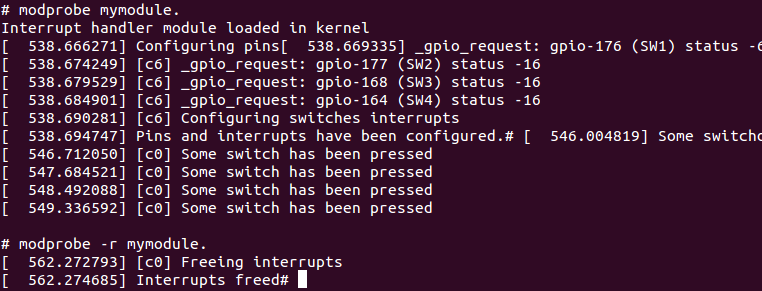
\includegraphics[width=16.5cm]{img/interrupt_success.png}
		\caption{Affichage du chargement du module, des pressions sur les boutons et de la suppression du module}
		\label{ser1ex9}
	\end{center}
\end{figure}
